\section{The deformed cells and the original group}
\label{cf:deformation}

\subsection{A mixed leaf and its two projection charts}
For real $x,t$ near $a,0$, put $E=e^{2\pi\ii x}$ and
$T=e^{2\pi\ii t}$. The mixed leaf has apex $\infty$ and ordered
quadrilateral
\begin{equation}\label{cf:mixed-leaf}
 (C_0,C_1,C_2,C_3)=(1,E/T,-1/T,-E).
\end{equation}
The successive half-arcs of its boundary circle are
$x-t,\,1/2-x,\,x+t,\,1/2-x$, all positive nearby.
Triangulation across $C_0C_2$ gives the triples
$(x-t,1/2-x,1/2+t)$ and
$(1/2-t,x+t,1/2-x)$.
Their complementary intermediate Lobachevsky terms cancel.
Using the normalized tetrahedron formula of
\cite[equation~(2.1)]{Geometry} gives exactly $\pi g(x,t)$.
This fixes the classical local constant.

\begin{figure}[ht]
\centering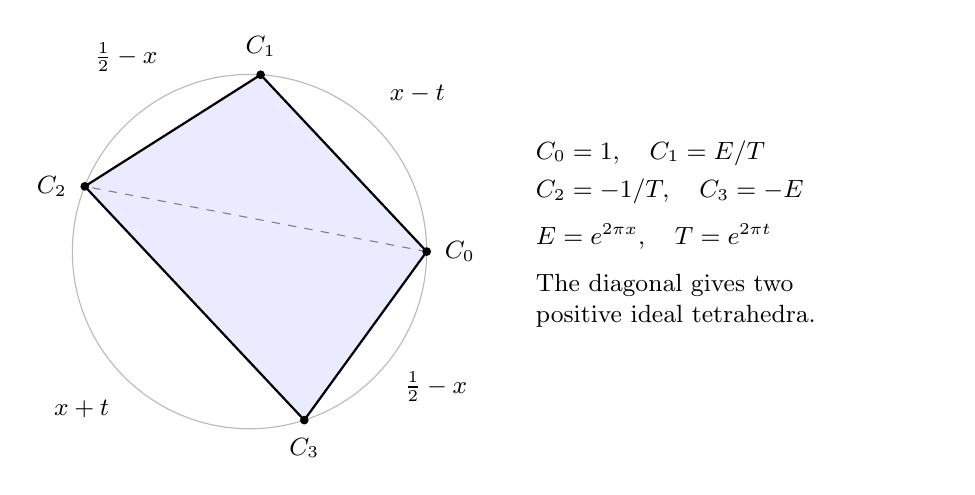
\begin{tikzpicture}[scale=2.25,every node/.style={font=\small}]
\coordinate(c0) at (1,0);
\coordinate(c1) at ({cos(86.4)},{sin(86.4)});
\coordinate(c2) at ({cos(158.4)},{sin(158.4)});
\coordinate(c3) at ({cos(288)},{sin(288)});
\draw[gray!55] (0,0) circle(1);
\fill[blue!8] (c0)--(c1)--(c2)--(c3)--cycle;
\draw[thick] (c0)--(c1)--(c2)--(c3)--cycle;
\draw[dashed,gray] (c0)--(c2);
\foreach \p/\lab/\pos in {c0/C_0/right,c1/C_1/above,c2/C_2/left,c3/C_3/below}
 {\fill(\p) circle(.7pt);\node[\pos=3pt] at(\p){$\lab$};}
\node at ({1.3*cos(43.2)},{1.3*sin(43.2)}) {$x-t$};
\node at ({1.3*cos(122.4)},{1.3*sin(122.4)}) {$\frac12-x$};
\node at ({1.3*cos(223.2)},{1.3*sin(223.2)}) {$x+t$};
\node at ({1.3*cos(324)},{1.3*sin(324)}) {$\frac12-x$};
\node[align=left,text width=5.1cm] at (2.75,.1)
 {$C_0=1,\quad C_1=E/T$\\[3pt]
  $C_2=-1/T,\quad C_3=-E$\\[6pt]
  $E=e^{2\pi\ii x},\quad T=e^{2\pi\ii t}$\\[6pt]
  The diagonal gives two\\positive ideal tetrahedra.};
\end{tikzpicture}

\caption{The boundary-plane coordinates of the mixed pyramid for
$x=0.30$, $t=0.06$. The apex is $\infty$.
The four successive half-arcs shown here are the actual parameters
of \eqref{cf:mixed-leaf}. At $t=0$ the quadrilateral becomes the
rectangle of the complete leaf.}
\label{cf:leaf-figure}
\end{figure}

Its ordered cross ratio and normalized fourth vertex are
\begin{equation}\label{cf:R}
\begin{split}
 \kap&=\frac{\sin\pi(x-t)\sin\pi(x+t)}{\cos^2\pi x}
                       =e^{-g_x},\\
 R&=\frac1{1+\kap}
    =\frac{\cos^2\pi x}{\cos^2\pi t}
    =\frac{T(1+E)^2}{E(1+T)^2}.
\end{split}
\end{equation}
Normalize its ordered base to $(0,\infty,1,R)$.
The plus-$t$ apex is
\begin{equation}\label{cf:flags}
 Z=\frac{1+E}{1+T},\qquad
 Z^2-(1+E)Z+ER=0.
\end{equation}
The other root is $TZ$, the apex of the minus-$t$ leaf in this
same normalization. The second projection chart is the reflected
minus-$t$ chart, whose apex is $Z/E$. It is not the reflection
of the plus-$t$ apex when $t\ne0$.

These formulas now define holomorphic projective coordinates
for complex $x,t$ near the complete point.
Reflection of coefficients is implemented by replacing the
phase variables by their reciprocals. Thus the reflected
minus apex is algebraically $Z/E$, without antiholomorphic
dependence on a parameter. Every defining face-map triple remains
pairwise distinct after shrinking the neighborhood; the two
auxiliary fixed points themselves coalesce at completeness.

\subsection{Whole complex face matching}
In the normalized chart the four white or completion maps are
\begin{equation}\label{cf:white}
\begin{aligned}
 W_0&=\begin{pmatrix}1&0\\0&E\end{pmatrix},&
 W_1&=\begin{pmatrix}1&E-1\\0&E\end{pmatrix},\\
 W_2&=\begin{pmatrix}E-R&R(1-E)\\E-1&1-ER\end{pmatrix},&
 W_3&=\begin{pmatrix}R&0\\1-E&ER\end{pmatrix}.
\end{aligned}
\end{equation}
The pure shaded map and the two odd cross-copy maps are
\begin{equation}\label{cf:shaded}
 S=\begin{pmatrix}0&-ER\\1&-1-E\end{pmatrix},\quad
 A=\begin{pmatrix}R&-R\\1&ER-1-E\end{pmatrix},\quad
 B=\begin{pmatrix}R/E-1-1/E&R\\-1&R\end{pmatrix}.
\end{equation}
All matrices are projective. For a mixed leaf, $W_0,W_2$
fix their two main corners and send $Z$ to $Z/E$.
The apex equation \eqref{cf:flags} verifies this last statement
also for $W_2$. The shaded assignments are
\[
 S:(Z,\infty,1)\mapsto(Z,0,R),\quad
 A:(Z,\infty,1)\mapsto(Z/E,R,0),\quad
 B:(Z,R,0)\mapsto(Z/E,\infty,1).
\]
Each is the map of the original labeled triangle.
The expressions $W_1,W_3$ are not extra leaf faces:
their actual white pieces come from its adjacent prism.

To check those pieces throughout the expression, keep the
original prism formula with complex wire parameters.
Write
\[
 \alpha=e^{2\pi\ii(z-x)},\quad
 \beta=e^{2\pi\ii(x+y-z)},\quad
 \gamma=e^{2\pi\ii(z-y)}.
\]
Its world coordinates are
\begin{equation}\label{cf:prism}
\begin{split}
 v_0&=1,\quad v_1=\alpha,\quad
 v_2=\alpha\beta,\quad v_3=\alpha\beta\gamma,\\
 P&=1+\alpha-
 \frac{\alpha[\alpha\beta(1+\gamma)-1-\alpha]}
                    {\alpha^2\beta^2\gamma-\alpha}.
\end{split}
\end{equation}
The lower, upper and output ordered quadrilaterals are
$(v_0,v_1,P,\infty)$, $(\infty,P,v_2,v_3)$ and
$(v_0,v_1,v_2,v_3)$, with wire phases
$\beta\gamma,\alpha\beta,\alpha\beta\gamma$.
For an ordered tuple $(a,b,c,d)$ let
\[
 M_{a,b,c}(z)=\frac{(z-a)(c-b)}{(z-b)(c-a)},\qquad
 R=M_{a,b,c}(d).
\]
Its world white maps are $M^{\#\, -1}W_jM$, where $\#$ reciprocates
$\alpha,\beta,\gamma$. At a real strict prism this agrees with
reflection; it is a holomorphic rational prescription in general.

The exact rational identities
\begin{equation}\label{cf:nine}
\begin{aligned}
 W_{F,1}=W_{G,1}=W_{o,1}&=W_{\rm top},&
 W_{F,3}=W_{G,3}=W_{o,3}&=W_{\rm bottom},\\
 W_{F,2}&=W_{G,0},&
 W_{o,0}=W_{F,0},\qquad W_{o,2}&=W_{G,2}
\end{aligned}
\end{equation}
are \cite[equation~(5.5)]{Geometry}. Their proof is a
rational substitution in three independent phase variables, so
it already proves \eqref{cf:nine} off the real chamber.
Here the top and bottom maps carry the original white triangles
$(P,v_1,v_2)$ and $(\infty,v_0,v_3)$ to their reflected charts.
No equality merely of absolute cross ratios is being used.

At an internal wire, \eqref{cf:local-differential} says that
the child output derivative is $g_x$ or the corresponding
stationary product derivative. The internal critical equations
therefore match the full complex cross ratios under the
same original vertex assignments as at completeness.
Three matched vertices fix a Möbius map, and the cross-ratio
equation matches the fourth. The former quadrilateral need not
remain planar; the argument matches its four flags and both
triangles of any fixed subdivision.

Turns and closure use
$T_Q(z)=(R-1)/(z-1)$ and $C_Q(z)=(z-R)/(z-1)$, with identities
\begin{equation}\label{cf:turn}
\begin{split}
 T_QW_{j+1}(E,R)&=W_j(E^{-1},1-R)T_Q,\\
 C_QW_j(E^{-1},R)&=W_{2-j}(E,R)C_Q .
\end{split}
\end{equation}
These are \cite[equation~(5.6)]{Geometry}, again rational
identities. Induction through \eqref{cf:nine} and
\eqref{cf:turn} proves that every triangular piece of a given
original white face has the same entire map. In particular the
parent prism supplies $W_1,W_3$ at every elementary cap edge.
The two completed root children ensure that the closing seams
are white. This is the specific place where the grammar
\eqref{cf:grammar} is retained.

\subsection{Relations and positivity on the retained chain}
Let $S^\#=S(E^{-1},R)$. Direct multiplication gives
\begin{equation}\label{cf:edge-words}
\begin{gathered}
 W_0S=S^\#W_0,\qquad W_2S=S^\#W_2,\qquad W_3S=S^\#W_1,\\
 W_0^{-1}BW_2^{-1}A=I,\quad
 W_2^{-1}BW_0^{-1}A=I,\quad
 W_1^{-1}BW_3^{-1}A=I.
\end{gathered}
\end{equation}
The first row is the pure edge return; the second is the odd
return, including its translational part. These are identities
for independent $E,R$, as proved in
\cite[equations~(5.7)--(5.8)]{Geometry}.
The original cut balls have a dual two-skeleton with generators
the paired faces and relations precisely these edge cycles and
the white seams. Since \eqref{cf:nine} identifies the whole
white maps, all those relations hold. The family is consequently
a representation of the original $\pi_1(Y^\eps_E)$.
The deformed image of a half ball is not assumed to be an
embedded convex polyhedron.

For later use, retain a compatible triangulation of the complete
cells. First perform the actual assembly to the single complete
polyhedron $P_E$. Its finitely many ideal vertices are distinct
by the incidence proof in \cite[Section~3]{Geometry}.
Choose an order on these vertices, and restrict it to every
constituent cell and its faces. The pulling triangulations agree
on internal quadrilaterals, since these are now the same labeled
face in $P_E$, regardless of the earlier turn or attachment order.
Coning from the first vertex to faces not containing it gives
nondegenerate tetrahedra. The vertex order chooses their diagonals;
each tetrahedron is oriented by the ambient oriented cell, rather
than by the increasing global vertex order. In that orientation
each complete shape is positive.
Use the identical subdivision in the second labeled copy.
All nontriangular external face pairings are the white maps
between corresponding copies, so their subdivisions match.
The pure and odd shaded pairings may permute vertices, but their
faces are already triangles and contain no diagonal to choose.
Thus no order on quotient cusp vertices, which could identify
many different cut vertices, is assumed.
Transport these finitely many vertices by the formulas above.
Their complete tetrahedra are positive, so their shapes remain
in the positive half-plane in one common small parameter
neighborhood. The full face maps match their triangles and
edge relations. We have the same oriented ideal fundamental
chain and the same peripheral marking as at completeness.
This construction does not require an ideal triangulation of
the subsequently filled manifold.

\section{Primitive logarithms and the unfilled cusps}
\label{cf:peripheral}

For a peripheral element fixing a selected flag, its similarity
multiplier means the coefficient of its affine action after
that flag is sent to $\infty$. At a finite flag $Z$ it is the
reciprocal of the derivative at $Z$. These are projective
similarity multipliers, twice the usual selected eigenvalue
logarithms. All logarithms below are their small branches,
zero at completeness.

The original disk and meridian words are the ones already
traced at completeness:
\begin{equation}\label{cf:peripheral-words}
 \lambda=W_2^{-1}W_0,\qquad
 \mu_0=S^{-1},\qquad
 \mu_-=A^{-1}W_0,\qquad
 \mu_+=W_0^{-1}B.
\end{equation}
They remain the same based curves in the original cut.
Their primitiveness and orientations are
\cite[equations~(7.1)--(7.5)]{Geometry}; in particular it is
the actual disk longitude, not a multiple read from an eigenvalue.
Their selected common flag is $Z$.
Put
\begin{equation}\label{cf:rhoQ}
 \rho=\frac{Z}{1+E-Z}=\frac1T,\qquad
 Q=\frac{E-Z}{Z-1}=\frac{ET-1}{E-T}.
\end{equation}
Inverting derivatives at $Z$ in
\eqref{cf:peripheral-words} gives the exact multipliers
\begin{equation}\label{cf:multipliers}
 \lambda:Q^2,\qquad
 \mu_0:\rho,\qquad
 \mu_-:\rho Q,\qquad
 \mu_+:\rho/Q.
\end{equation}
For example the fixed-point equation of $S$ is precisely
\eqref{cf:flags}, and substitution in the Möbius derivative
$\det S/(cZ+d)^2$ gives the first meridian factor.
The same substitution gives the other three factors.
At $t=0$ both $\rho$ and $Q$ equal one, so no central logarithmic
constant can enter their small branches.

From \eqref{cf:g} and \eqref{cf:rhoQ} one has
$Q=e^{-v}$ and $\rho=e^{-2\pi\ii t}$.
It follows that the original signed meridian and disk longitude
have logarithms
\begin{equation}\label{cf:primitive-logs}
 U=-2\pi\ii t+\eps v=-2\pi\ii\chi,\qquad V=-2v.
\end{equation}
Using the envelope rule proves \eqref{cf:UV}.
The half-twist part of $G=2\pi\ii\Phi_\eps$ is
$-\eps V^2/8$ at each leaf, exactly the shear in
\eqref{cf:local-potential}.

All main cusps also retain their actual peripheral words.
At corner $C_j$ the small main meridian is
$W_{j-1}^{-1}W_j$, or its inverse according to orientation.
Both factors fix that corner. Their derivatives are equal:
$E^{-1}$ at $C_0,C_2$ and $E$ at $C_1,C_3$, using the
finite coordinate at infinity. Thus the meridian multiplier
is identically one. It is nonidentity at the complete point,
and remains so nearby; hence it is parabolic.
Every element commuting with a nonidentity parabolic Möbius
map is a translation in its fixed-flag chart.
The original main longitude commutes with this meridian.
Its multiplier is therefore also one. This verifies
the entire unfilled main peripheral group, not just a
trace equation at a single corner.

The selected auxiliary flags, the main flags and all face
maps vary holomorphically and stay in bounded frames near
their complete values. A finite collection of charts suffices.
We may therefore choose one neighborhood where the actual
framed family and all the positive tetrahedra constructed above
are simultaneously defined.
